% chapters/08_user_manual.tex
\chapter{用户手册与部署指南}

\section{概述}

本章为开发者提供完整的部署指南，帮助用户从零开始搭建开发环境、编译星绽内核、配置启动参数并验证 dm-crypt 与 dm-verity 的功能。所有步骤均已在 Ubuntu 24.04 上验证通过。

\section{运行环境准备}

\subsection{宿主机要求}

推荐使用以下环境进行开发和测试：

\begin{itemize}
    \item \textbf{操作系统}：Ubuntu 24.04 LTS
    \item \textbf{架构}：x86\_64
    \item \textbf{内存}：至少 8 GiB
    \item \textbf{磁盘空间}：至少 20 GiB
\end{itemize}

\subsection{依赖工具安装}

\begin{table}[H]
    \centering
    \caption{开发环境依赖}
    \label{tab:dev_dependencies}
    \begin{tabular}{p{0.25\textwidth}p{0.25\textwidth}p{0.40\textwidth}}
        \toprule
        \textbf{依赖项} & \textbf{版本要求} & \textbf{用途} \\
        \midrule
        Rust / Cargo & 1.75.0+ & 核心语言工具链 \\
        QEMU & 8.2.2+ & 硬件虚拟化 \\
        Docker & 29.4.3+ & 容器化构建环境 \\
        星绽镜像 & asterinas/asterinas:0.18.0-20260618 & 官方工具链 \\
        Clang / LLVM & 18.0.0+ & 内核编译 \\
        \bottomrule
    \end{tabular}
\end{table}

\section{快速开始：用户态演示}

\subsection{运行测试套件}

\begin{verbatim}
cargo test
\end{verbatim}

\subsection{演示透明加密}

\begin{verbatim}
cargo run -p dmctl -- demo-crypt
\end{verbatim}

\subsection{演示完整性校验}

\begin{verbatim}
cargo run -p dmctl -- demo-verity
\end{verbatim}

\section{星绽内核集成}

\subsection{构建内核}

\begin{verbatim}
docker run --rm --privileged --network=host \
  -v asterinas-src:/root/asterinas \
  -w /root/asterinas \
  asterinas/asterinas:0.18.0-20260618 make kernel
\end{verbatim}

\subsection{构建受保护的根文件系统镜像}

\begin{verbatim}
# dm-crypt 加密镜像
./scripts/build_crypt_rootfs.sh

# dm-verity 校验镜像
./scripts/build_verity_rootfs.sh
\end{verbatim}

\section{系统运行与参数配置}

\subsection{QEMU 启动命令}

\begin{verbatim}
qemu-system-x86_64 \
  -kernel artifacts/asterinas-kernel \
  -initrd artifacts/initramfs \
  -drive file=target/verity-rootfs.img,format=raw,if=virtio \
  -append "root=/dev/vda console=ttyS0"
\end{verbatim}

\subsection{内核启动参数配置}

启用 dm-verity：

\begin{verbatim}
rootfs_verity.scheme=dm-verity rootfs_verity.hash=<64-char-root-hash>
\end{verbatim}

启用 dm-crypt：

\begin{verbatim}
dm_crypt.device=/dev/vda dm_crypt.key=<128-char-hex-key>
\end{verbatim}

\begin{figure}[H]
    \centering
    \includegraphics[width=0.9\textwidth]{figures/root_protection_init.png}
    \caption{根保护初始化序列图}
    \label{fig:root_init}
\end{figure}

启动流程的关键阶段：
\begin{enumerate}
    \item QEMU 加载星绽内核和 initramfs。
    \item 内核解析命令行参数，构建 DmBootConfig。
    \item aster-dm 组件初始化映射器链（VirtioBlkAdapter 到 DmCryptDevice 到 DmVerityDevice）。
    \item 执行 self\_test\_ext2\_magic 自检。
    \item initramfs 执行 pivot\_root 切换到受保护根文件系统。
    \item 系统进入用户态。
\end{enumerate}

\begin{figure}[H]
    \centering
    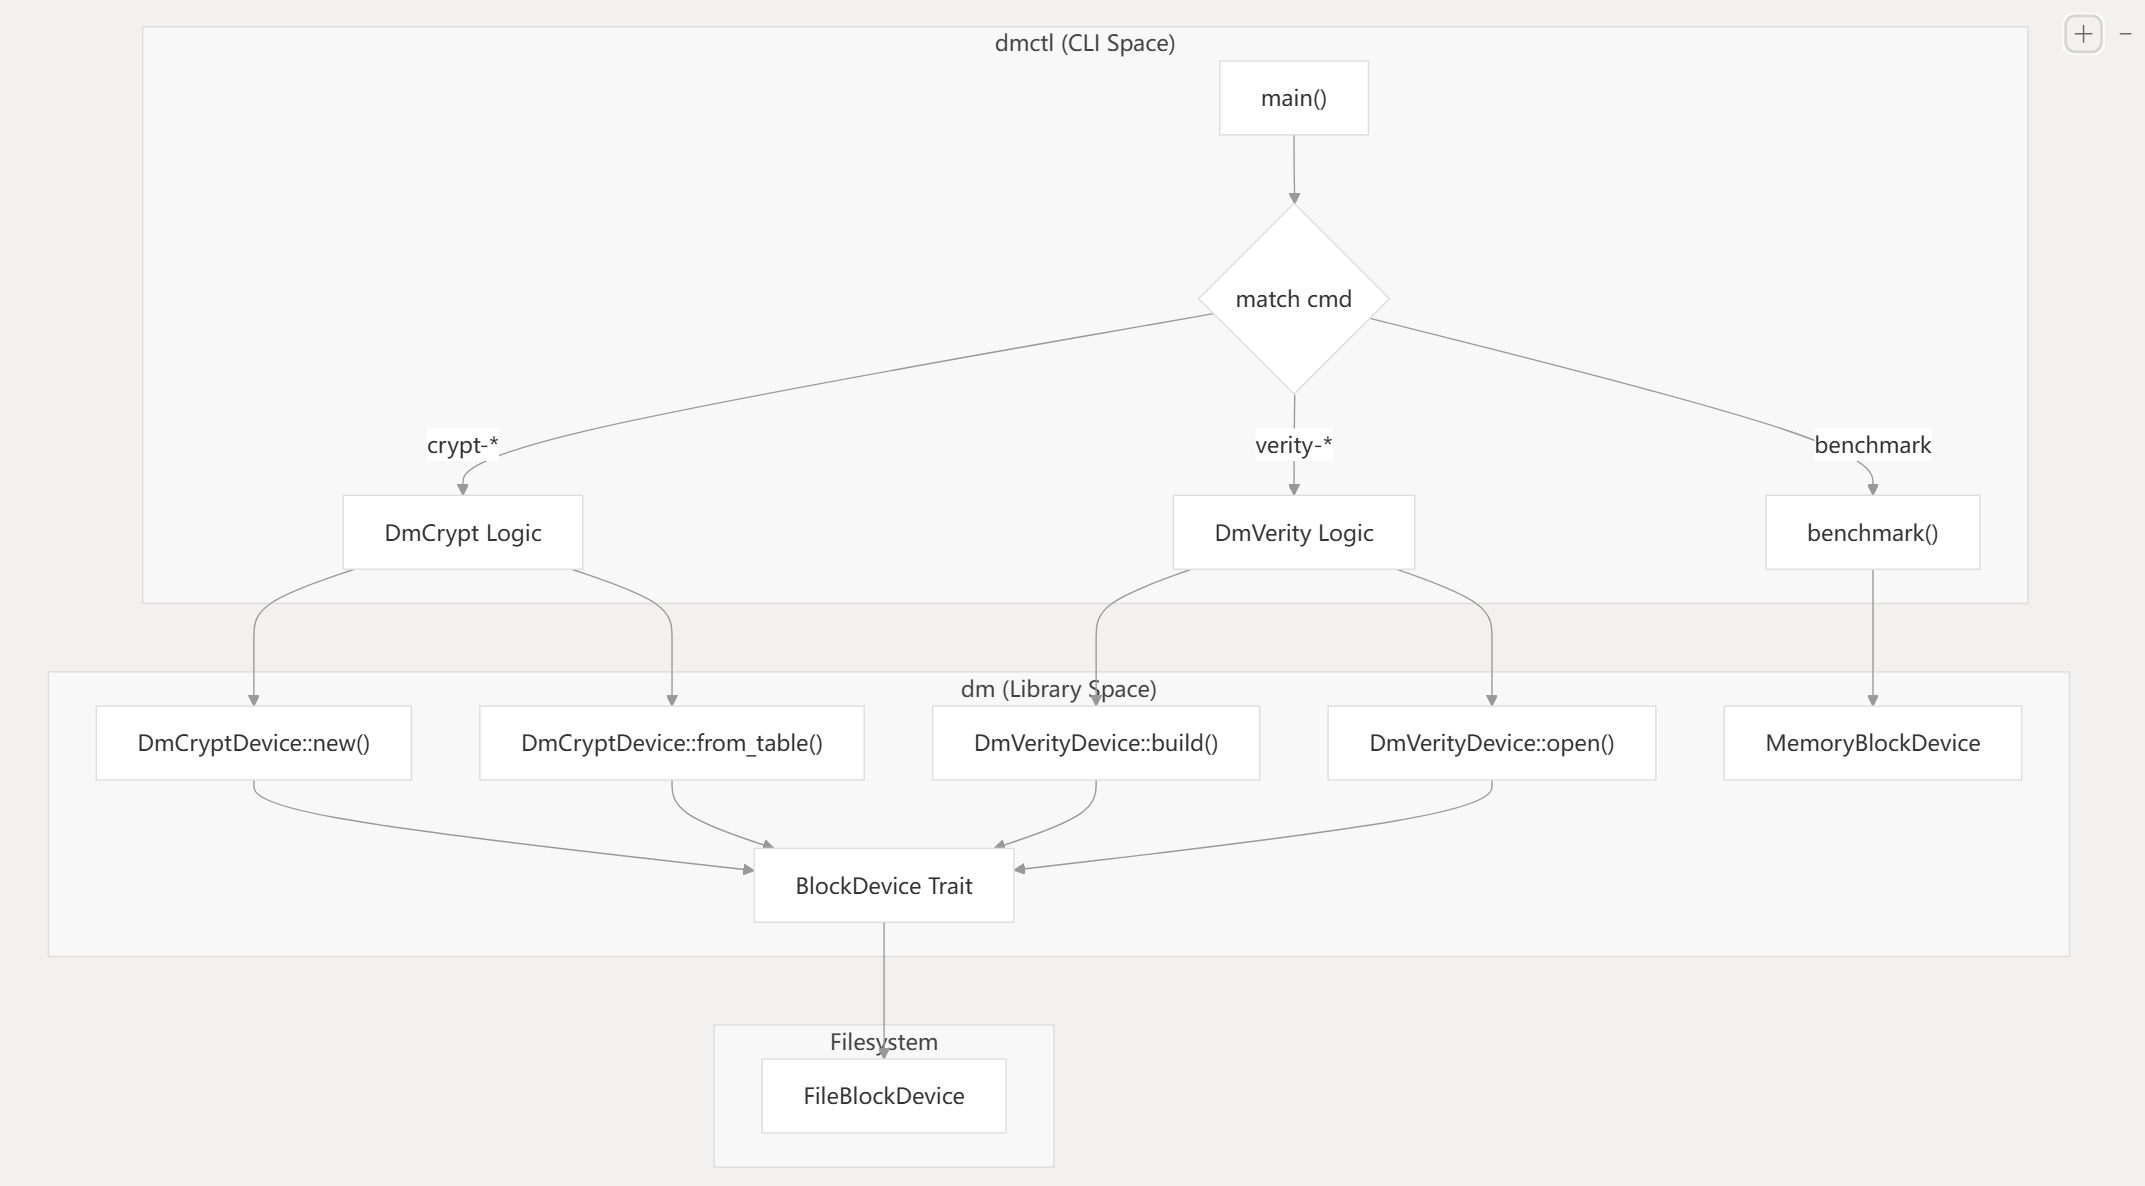
\includegraphics[width=0.9\textwidth]{figures/dmctl_command_flow.png}
    \caption{dmctl 命令执行流程图}
    \label{fig:dmctl_flow}
\end{figure}

\section{小结}

本章提供了完整的用户手册与部署指南，涵盖了从环境准备、代码编译、镜像构建到系统运行的全流程。通过遵循本章的步骤，开发者可以快速验证核心功能并部署星绽内核。